\documentclass[twoside]{article}
\usepackage[left=3cm, right=2cm, top=3cm, bottom=2cm]{geometry}
\usepackage{babel}
\usepackage[utf8]{inputenc}
\usepackage{amsmath, amssymb, amsfonts}
\usepackage{mathtools}
\usepackage{mathrsfs}
\usepackage{siunitx}
\usepackage{fancyhdr}
\usepackage{xcolor}
\usepackage{graphicx}
\usepackage{enumitem}
\usepackage{booktabs}
\usepackage{longtable}
\usepackage{array}
\usepackage{multirow}
\usepackage{wrapfig}
\usepackage{float}
\usepackage{colortbl}
\usepackage{pdflscape}
\usepackage{tabu}
\usepackage{threeparttable}
\usepackage{threeparttablex}
\usepackage[normalem]{ulem}
\usepackage{makecell}
\usepackage{tikz}
%\usetikzlibrary{patterns,snakes}



% Redefinir o comando \section para ter o mesmo tamanho que \subsection
\makeatletter
\renewcommand\section{\@startsection{section}{1}{\z@}%
                                     {-3.5ex \@plus -1ex \@minus -.2ex}%
                                     {2.3ex \@plus.2ex}%
                                     {\normalfont\large\bfseries}}
\makeatother


% Metadados
\title{Título}

\author{author}

\newcommand{\booktitle}{Cálculo e Álgebra Linear}

\newcommand{\booksubtitle}{: Vol 1: Vetores no plano e funções de uma variáve.}


\newcommand{\bookauthors}{Kaplan, W.; Lewis, D. J.}

\newcommand{\bookaddres}{Rio de Janeiro}

\newcommand{\bookpublisher}{Ed. Univ, de Brasilia}

\newcommand{\bookyear}{1972}

\newcommand{\chaptertitle}{Introdução}

\newcommand{\chapternumber}{0}

% Define a cor principal do arquivo
\definecolor{mainColor}{HTML}{5b017d}



% Definir leftmargin=* para todos os ambientes enumerate
\setlist[enumerate,1]{leftmargin=*, label=\textbf{\arabic*.}}


% Bold Vector
\newcommand{\vet}[1]{\mathbf{\hat{#1}}}

% Comando iniciar Solução
\newcommand{\iniSol}{
    \noindent\textcolor{mainColor}{\rule{0.3\textwidth}{0.4pt}}\\
    \noindent\textcolor{mainColor}{\textbf{Solução:}}\\
}

% Comando finalizar Solução
\newcommand{\fimSol}{
    %
    \hfill\fcolorbox{mainColor}{mainColor}

    
    \hfill\textcolor{mainColor}{\rule{0.3\textwidth}{0.4pt}}
}

% Configuração do cabeçalho e rodapé
\pagestyle{fancy}
\fancyhf{} % Limpa os cabeçalhos e rodapés atuais

% Cabeçalho para páginas pares
\fancyhead[RE]{Igo da Costa Andrade}

% Cabeçalho para páginas ímpares
\fancyhead[LO]{
        Solucionário de 
    Cálculo e Álgebra Linear
        (Kaplan, W.; Lewis, D. J.)
        }

\fancyhead[RO]{
    
}

% Número da página no rodapé (centrado)
\fancyfoot[C]{\thepage}

% Ajuste para reconhecimento de código python


% Novo comando para a criação do cabeçalho personalizado
\newcommand{\makeheader}{
  \textcolor{mainColor}{\hrule}
  \vspace{0.25cm}
  \begin{minipage}[c]{12cm}
    \begin{center}
      Resolução de Problemas do Livro\\
      \vspace{0.25cm}
      \textcolor{mainColor}{\large{\textbf{Cálculo e Álgebra Linear: Vol 1: Vetores no plano e funções de uma variáve. (Kaplan, W.; Lewis, D. J.)}}}\\
      \vspace{0.7cm}
      \small{por}\\
      \vspace{0.2cm}
      \textbf{\large{Igo da Costa Andrade}}
    \end{center}
    \vspace{0.25cm}
    \hrule
    \vspace{0.25cm}
    \textbf{Referência}
  
    \uppercase{Kaplan, W.; Lewis, D. J.}. \textbf{Cálculo e Álgebra Linear}: Vol 1: Vetores no plano e funções de uma variáve.. Rio de Janeiro, Ed. Univ, de Brasilia, 1972.
  \end{minipage}
  \begin{minipage}[c]{4cm}
    \begin{flushright}
      \includegraphics[width=0.8\linewidth]{figure/capa.png}    
    \end{flushright}
  \end{minipage}
  \vspace{0.25cm}
  \textcolor{mainColor}{\hrule}
  
  \begin{center}
    \vspace{0.5cm}
        \large{\textbf{Capítulo 0: }}
            \large{\textbf{Introdução}}
        \vspace{0.5cm}
  \end{center}
}


\begin{document}
\thispagestyle{empty}

\makeheader


\section*{PROBLEMAS}

\begin{enumerate}
  \item 
  \begin{enumerate}[label=(\alph*)]
    \item Encontre um inteiro $x$ tal que $10 \sqrt{2} < x < 10\sqrt{3}$.\\
    \iniSol
      Observemos que $10\sqrt{2}$, $x$ e $10\sqrt{3}$ são números positivos. Então:
      \begin{itemize} 
      \item Pela primeira desigualdade, temos:
      \begin{align*}
      10\sqrt{2} < x &\Rightarrow
      \begin{cases}
        (10\sqrt{2})\cdot (10\sqrt{2}) < (10\sqrt{2}) \cdot x\\
        (10\sqrt{2})\cdot x < x\cdot x
      \end{cases}
      \Rightarrow
      \begin{cases}
        200 < (10\sqrt{2}) \cdot x\\
        (10\sqrt{2}) \cdot x < x^2
      \end{cases}
      \\
      &\Rightarrow 200 < x^2
      \end{align*}
      %%
      \item Pela segunda desigualdade, temos:
      \begin{align*}
        x < 10 \sqrt{3} & \Rightarrow
        \begin{cases}
          x \cdot x < (10\sqrt{3}) \cdot x \\
          (10\sqrt{3}) \cdot x < (10\sqrt{3}) \cdot (10 \sqrt{3})
        \end{cases}
        \Rightarrow
        \begin{cases}
          x^2 < (10\sqrt{3}) \cdot x\\
          (10\sqrt{3}) \cdot x < 300
        \end{cases}
        \\
        &\Rightarrow x^2 < 300
      \end{align*}
      \end{itemize}
      %%
      Combinando os resultados acima, obtemos:
      \begin{align*}
      10\sqrt{2} < x < 10\sqrt{3} \Rightarrow 200 < x^2 < 300 &\Rightarrow x^2 = 225, 256, 289\\
      &\Rightarrow x = 15, 16, 17.
      \end{align*}
    \fimSol
    %%%%
    \item Encontre um inteiro $x$ tal que $-5\sqrt{2} < x < -3\sqrt{3}$.\\
    \iniSol
      Observememos que $-5\sqrt{2}$, $x$ e $-3\sqrt{3}$ são todos números negativos.
      \begin{itemize}
        \item Pela primeira desigualdade:
        \begin{align*}
          -5\sqrt{2} < x &\Rightarrow 
          \begin{cases}
          (-5\sqrt{2}) \cdot (-5\sqrt{2}) > (-5\sqrt{2}) \cdot x\\
          (-5\sqrt{2}) \cdot x > x^2
          \end{cases}
          \Rightarrow
          \begin{cases}
            50 > (-5\sqrt{2}) \cdot x\\
            (-5\sqrt{2}) \cdot x > x^2
          \end{cases}
          \\
          &\Rightarrow 50 > x^2
        \end{align*}
        %%
        \item Pela segunda desigualdade,
        \begin{align*}
          x < -3\sqrt{3} &\Rightarrow
          \begin{cases}
            x \cdot x > (-3\sqrt{3})\cdot x\\
            (-3\sqrt{3}) \cdot x> (-3\sqrt{3}) \cdot (-3\sqrt{3}) 
          \end{cases}
          \Rightarrow 
          \begin{cases}
            x^2 > (-3\sqrt{3}) \cdot x\\
            (-3\sqrt{3}) \cdot x > 27
          \end{cases}
          \\
          &\Rightarrow x^2 > 27
        \end{align*}
      \end{itemize}
      %%
      Combunando os resultados acima, tem-se:
      \begin{align*}
        -5\sqrt{2} < x < -3\sqrt{3} \Rightarrow 50 > x^2 > 27 & \Rightarrow x^2 = 49\;\text{ou}\;36 \\&\Rightarrow
        x^2 = (-7)^2\;\text{ou}\;(-6)^2\\
        &\Rightarrow x = -7\;\text{ou}\;-6
      \end{align*}
    \fimSol
    %%%%
    \item Encontre um número racional $x$ tal que $\sqrt{2} < x < \sqrt{3}$.\\
    \iniSol
      \begin{align*}
        \sqrt{2} < x < \sqrt{3} &\Rightarrow (\sqrt{2})^2 < x^2 < (\sqrt{3})^2 \Rightarrow 2 < x^2 < 3
      \end{align*}
      A título de exemplo, façamos:
      \begin{align*}
        \sqrt{2} < x < \sqrt{3} &\Rightarrow 2 < x^2 < 3 \Rightarrow \dfrac{200}{100} < x^2 < \dfrac{300}{100} \\
        &\Rightarrow
        x^2 = \dfrac{225}{100}, \dfrac{256}{100}, \;\text{ou}\:\dfrac{289}{100} \Rightarrow x^2 = \left(\dfrac{15}{10}\right)^2, \left(\dfrac{16}{10}\right)^2, \;\text{ou}\:\left(\dfrac{17}{10}\right)^2 \\
        &\Rightarrow x = \dfrac{15}{10}, \dfrac{16}{10}, \;\text{ou}\:\dfrac{17}{10} 
      \end{align*}
    \fimSol
    %%%%
    \item Encontre um  número racional $x$ tal que $\pi < x < \pi + 0.01$.\\
    \iniSol
      $x = 3,14$
    \fimSol
    \end{enumerate}
    %%%%
    \item Determine se $x < y$, $x = y$, ou $x < y$ para cada um dos seguintes casos:
    \begin{enumerate}[label=(\alph*)]
      \item $x=-3$, $y = -2$
      \item $x = 1$, $y = -2$
      \item $x = \sqrt{5} - \sqrt{3}$, $y = \sqrt{7} - \sqrt{2}$
      \item $x = \dfrac{1}{\sqrt{3} - \sqrt{11}}$, $y = \dfrac{1}{\sqrt{3} - \sqrt{13}}$
    \end{enumerate}
    \iniSol
    \begin{enumerate}[label=(\alph*)]
      \item $x=-3$, $y = -2$
        \begin{align*}
          x - y = -3 - (-2) = -3 + 2 = -1 < 0 \Rightarrow x < y
        \end{align*}
      %%
      \item $x = 1$, $y = -2$
      \begin{align*}
        x - y = 1 - (-2) = 1 + 2 = 3 > 0 \Rightarrow x > y
      \end{align*}
      %%
      \item $x = \sqrt{5} - \sqrt{3}$, $y = \sqrt{7} - \sqrt{2}$
      \begin{align*}
        y - x &= (\sqrt{7} - \sqrt{2}) - (\sqrt{5} - \sqrt{3}) = \sqrt{7} - \sqrt{2} - \sqrt{5} + \sqrt{3}\\
        &= \sqrt{7} - \sqrt{5} + \sqrt{3} - \sqrt{2} = (\sqrt{7} - \sqrt{5}) + (\sqrt{3} - \sqrt{2})
      \end{align*}
      Como $\sqrt{7}- \sqrt{5} > 0$ e $\sqrt{3} - \sqrt{2}> 0$, então:
      \begin{align*}
        (\sqrt{7} - \sqrt{5}) + (\sqrt{3} - \sqrt{2}) > 0 \Rightarrow y - x > 0 \Rightarrow y > x \Rightarrow x < y
      \end{align*}
      %%
      \item $x = \dfrac{1}{\sqrt{3} - \sqrt{11}}$, $y = \dfrac{1}{\sqrt{3} - \sqrt{13}}$\\
      %%
      Façamos $u = \dfrac{1}{x} = \sqrt{3} - \sqrt{11}$ e $v = \dfrac{1}{y} = \sqrt{3} - \sqrt{13}$. Então,
      \begin{align*}
        &u - v = (\sqrt{3} - \sqrt{11}) - (\sqrt{3} - \sqrt{13}) = \sqrt{3} - \sqrt{11} - \sqrt{3} + \sqrt{13}
        = \sqrt{13} - \sqrt{11} > 0\\ \Rightarrow & u > v \Rightarrow \dfrac{1}{x} > \dfrac{1}{y} \Rightarrow x < y
      \end{align*}
    \end{enumerate}
    \fimSol
    %%%%
    \item Calcule: (a) $|-3.5|$, (b) $|0,2|$, (c) $||x||$, (d) $|-|x||$, (e) $|x-y| - |y-x|$\\
    \iniSol
    \begin{enumerate}[label=(\alph*)]
      \item $|-3.5| = 3.5$
      \item $|0,2| = 0,2$
      \item $||x|| = |x|$
      \item $|-|x|| = |-1| \cdot |x| = 1 \cdot |x| = |x|$
      \item $|x-y| - |y-x| = |x-y| - |-(x-y)| = |x-y| - |-1|\cdot|x-y| = |x-y| - |x-y| = 0$
    \end{enumerate}
    \fimSol
    %%%%
    \item Mostre que $|a-b|$ pode ser interpretado como a distância entre $a$ e $b$ sobre o eixo dos números.\\
    \iniSol
      No caso em que $a = b$, $|a-b| = 0$ que é a distãncia entre $a$ e $b$.
      %%
      Caso $a > b$:
      \begin{itemize}
        \item $a > b > 0 \Rightarrow |a-b| = a-b$
        \begin{figure}[H]
          \centering
          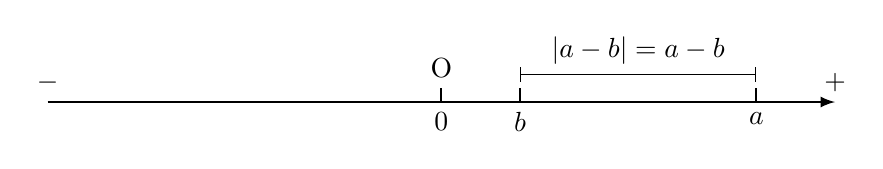
\begin{tikzpicture}
            \draw[-latex, thick] (-5, 0) node[above] {$-$} -- (5, 0) node[above] {$+$};
            \draw[thick] (0, 5pt) node[above] {O} -- (0, 0) node[below] {$0$};
            \draw[thick] (1, 5pt) -- (1, 0) node[below] {$b$};
            \draw[thick] (4, 5pt) -- (4, 0) node[below] {$a$};
            \draw [|-|] (1, 10pt) -- (4, 10pt) node[midway, above] {$|a-b| = a-b$};
          \end{tikzpicture}
        \end{figure}
        %%
        \item $a > b = 0 \Rightarrow |a-b| = |a-0| = |a| = a$
        \begin{figure}[H]
          \centering
          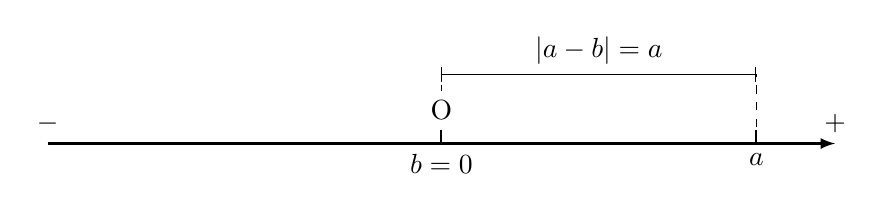
\begin{tikzpicture}
            \draw[thick] (0, 5pt) -- (0, 0) node[below] {$b = 0$};
            \draw[thick] (4, 5pt) -- (4, 0) node[below] {$a$};
            \draw [|-|] (0, 25pt) -- (4, 25pt) node[midway, above] {$|a-b| = a$};
            \draw[dashed] (0,0) -- (0, 25pt);
            \draw[dashed] (4,0) -- (4, 25pt);
            \draw[-latex, thick] (-5, 0) node[above] {$-$} -- (5, 0) node[above] {$+$};
            \draw[thick] (0, 5pt) node[above, fill=white] {O} -- (0, 0);
          \end{tikzpicture}
        \end{figure}
        %%
        \item $a > 0 > b$. Façamos $b = -|b|$, em que $|b|$ é a distância entre $b$ e o zero da reta numérica. Então: $|a-b| = |a - (-|b|)| = |a + |b|| = a + |b|$
        \begin{figure}[H]
          \centering
          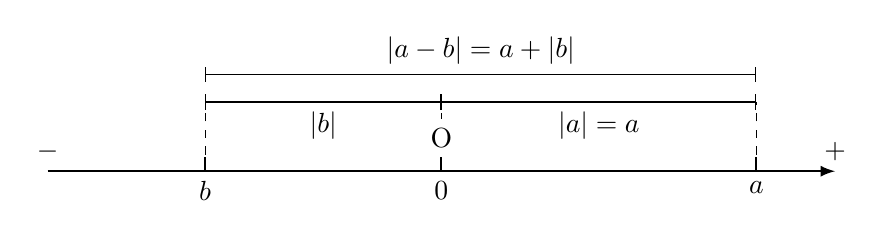
\begin{tikzpicture}
            \draw[thick] (-3, 5pt) -- (-3, 0) node[below] {$b$};
            \draw[thick] (4, 5pt) -- (4, 0) node[below] {$a$};
            \draw [|-|] (0, 25pt) -- (4, 25pt) node[midway, below] {$|a| = a$};
            \draw [|-|] (0, 25pt) -- (-3, 25pt) node[midway, below] {$|b|$};
            \draw[dashed] (0,0) -- (0, 25pt);
            \draw[dashed] (4,0) -- (4, 25pt);
            \draw[dashed] (-3, 0) -- (-3, 25pt);
            \draw[|-|] (-3, 35pt) -- (4, 35pt) node[midway, above] {$|a-b| = a + |b|$};
            \draw[-latex, thick] (-5, 0) node[above] {$-$} -- (5, 0) node[above] {$+$};
            \draw[thick] (0, 5pt)  node[above, fill=white] {O} -- (0, 0) node[below] {$0$};
          \end{tikzpicture}
        \end{figure}
        %%
        \item $a = 0 > b$. Então: $|a-b| = |0 - b| = |-b| = |b|$, em que $|b|$ é a distância entre $b$ e o zero da reta numérica, que neste caso, é a posição de $a$.
        \begin{figure}[H]
          \centering
          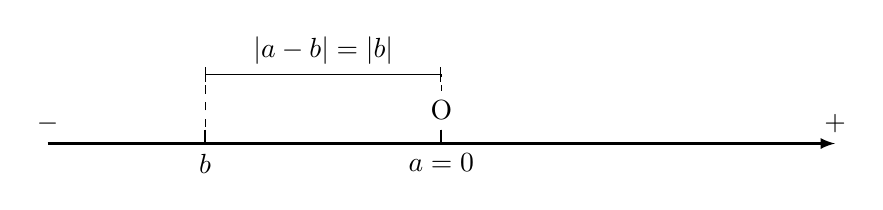
\begin{tikzpicture}
            \draw[thick] (-3, 5pt) -- (-3, 0) node[below] {$b$};
            \draw[thick] (0, 5pt) -- (0, 0) node[below] {$a=0$};
            \draw [|-|] (-3, 25pt) -- (0, 25pt) node[midway, above] {$|a-b| = |b|$};
            \draw[dashed] (-3,0) -- (-3, 25pt);
            \draw[dashed] (0,0) -- (0, 25pt);
            \draw[-latex, thick] (-5, 0) node[above] {$-$} -- (5, 0) node[above] {$+$};
            \draw[thick] (0, 5pt) node[above, fill=white] {O} -- (0, 0);
          \end{tikzpicture}
        \end{figure}
        %%
        \item $0 > a > b$. Façamos $a = -|a|$ e $b = -|b|$. Então: $|a-b| = |-|a| - (-|b|)| = |-|a| + |b|| = ||b| - |a|| = |b| - |a|$, pois $0 < |a| < |b|$.
        \begin{figure}[H]
          \centering
          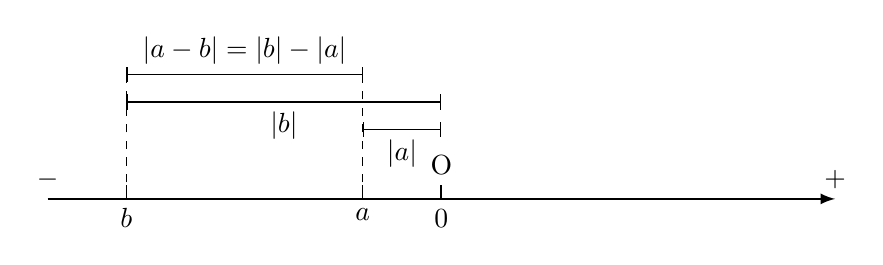
\begin{tikzpicture}
            \draw (-1, 5pt) -- (-1, 0) node[below] {$a$};
            \draw [|-|] (0, 25pt) -- (-1, 25pt) node[below, midway] {$|a|$};
            \draw[dashed] (-1, 0) -- (-1, 45pt);
            \draw (-4, 5pt) -- (-4, 0) node[below] {$b$};
            \draw[|-|] (0, 35pt) -- (-4, 35pt) node[below, midway] {$|b|$};
            \draw[dashed] (-4, 0) -- (-4, 45pt);
            \draw[|-|] (-1, 45pt) -- (-4, 45pt) node[midway, above] {$|a-b| = |b|-|a|$};
            \draw[-latex, thick] (-5, 0) node[above] {$-$} -- (5, 0) node[above] {$+$};
            \draw[thick] (0, 5pt) node[above, fill=white] {O} -- (0, 0) node[below] {$0$};
          \end{tikzpicture}
        \end{figure}
      \end{itemize}
      Os casos em que $b > a$ podem ser determinados de forma análoga, bastando lembrar que $|a-b| = |-(b-a)| = |b-a|$ e repetir o aciocínio acima.
    \fimSol
    %%%%
    \item Achar $x$ em cada um dps casos: (a) $|x| = 0$, (b) $|x| = 2$, (c) $|x-1| = 2$, (d) $|x+1| = 1$.\\
    \iniSol
    \begin{enumerate}[label=(\alph*)]
      \item $|x|=0 \Rightarrow = x = 0$
      \item $|x| = 2 \Rightarrow x = -2$ ou $x = 2$.
      \item 
      \begin{align*}
        |x-1| = 2 \Rightarrow 
        \begin{cases}
          x-1 = -2\\
          x-1 = 2
        \end{cases}
        \Rightarrow
        \begin{cases}
          x = -1\\
          x = 3
        \end{cases}
      \end{align*}
      %%
      \item
      \begin{align*}
        |x+1| = 1 \Rightarrow 
        \begin{cases}
          x+1 = -1\\
          x+1 = 1
        \end{cases}
        \Rightarrow
        \begin{cases}
          x = 2\\
          x = 0
        \end{cases}
      \end{align*}
    \end{enumerate}
    \fimSol
    \item O símbolo $\sqrt{x}$ indica $0$ se $x=0$ e a raiz quadrada positiva de $x$, se $x > 0$. Justifique as seguintes regras para todos reais $x$ e $y$.
    \begin{enumerate}[label=(\alph*)]
      \item $\sqrt{x^2} = |x|$\\
      \iniSol
        Se $x = 0$, a identidade é imediada.\\
        Se $x > 0$, então $\sqrt{x^2} = x = |x|$.\\
        Se $x < 0$, então $-x > 0$. Assim, $\sqrt{x^2} = \sqrt{(-x)^2} = -x = |x|$.\\
        Portanto, para todo número real $x$, vale $\sqrt{x^2} = |x|$.
      \fimSol
      %%
      \item $\sqrt{x^4} = x^2$\\
      \iniSol
        Inicialmente, observemos que para todo $x \in \mathrm{R}$, tem-se que $x^2 > 0$. Assim,
        $$
        \sqrt{x^4} = \sqrt{(x^2)^2} = x^2.
        $$
      \fimSol
      %%
      \item $(x|x|)^2 = x^4$\\
      \iniSol
        Se $x = 0$ o resultado é imediatamente verdadeiro.\\
        Se $x > 0$, temos que $|x| = x$. Nesse caso,
        $$
        (x|x|)^2 = (x \cdot x)^2 = (x^2)^2 = x^4.
        $$
        Se $x < 0$, temos que $|x| = -x$. Nesse caso,
        $$
        (x|x|)^2 = \left[x \cdot (-x)\right]^2 = (-x^2)^2 = (x^2)^2 = x^4.
        $$
        Portanto, para qualquer $x$ real, vale $(x|x|)^2 = x^4$.
      \fimSol
      %%
      \item $\sqrt{x^2 - 2xy + y^2} = |x-y|$.\\
      \iniSol
        Se $x = y$, a identidade é imediatamente válida.\\
        Se $x > y$ ($\Rightarrow x - y > 0$),  então
        \begin{align*}
          \sqrt{x^2 - 2xy + y^2} = \sqrt{(x-y)^2} = x-y = |x-y|.
        \end{align*}
        Se $x < y$ ($\Rightarrow x - y < 0 \Rightarrow -(x-y) > 0$), então
        \begin{align*}
          \sqrt{x^2 - 2xy + y^2} = \sqrt{\left[-(x-y)\right]^2} = -(x-y) = |x-y|.
        \end{align*}
        Portanto, para quaisquer $x$ e $y$ reais vale $\sqrt{x^2 - 2xy + y^2} = |x-y|$.
      \fimSol
    \end{enumerate}
    \item Mostre que as regras 20 e 21 são válidas para todos os números reais $a$ e $b$.\\
    \iniSol
      \begin{itemize}
        \item Regra 20: $|a| = |-a|$.\\
        Sem perda de generalidade, seja $a > 0$, donde $-a < 0$. Então, $|a| = a$ e $|-a| = -(-a) = a$. Logo, $|a| = |-a|$.
        \item Regra 21: $|ab| = |a||b|$.\\
        Caso I: $a \leq 0$ ($\Rightarrow |a| = a$)  e $b \leq 0$ ($\Rightarrow |b| = b$). Então:
        \begin{align*}
          ab \leq 0 \Rightarrow |ab| = ab = |a||b|.
        \end{align*}
        Caso II: $a \leq 0$ ($\Rightarrow |a| = a$) e $b < 0$ ($\Rightarrow |b| = -b$). Então:
        \begin{align*}
          ab < 0 \Rightarrow |ab| = -(ab) = a \cdot (-b) = |a||b|.
        \end{align*}
        Caso III: $a < 0$ ($\Rightarrow |a| = -a$) e $b < 0$ ($\Rightarrow |b| = -b$). Então:
        \begin{align*}
          ab > 0 \Rightarrow |ab| = ab = (-a)(-b) = |a||b|.
        \end{align*}
        Portanto, para quaisquer reais $a$ e $b$, vale $|ab| = |a||b|$.
      \end{itemize}
    \fimSol
    \item 
    \begin{enumerate}[label=(\alph*)]
      \item $a < b$ implica $a^2 < b^2$?\\
      \iniSol
      Não. Basta tomarmos como contra-exemplo $a = -2$ e $b = -1$, donde $a < b$, mas $a^2 > b^2$.
      \fimSol
      \item $a < b$ implica $a^3 < b^3$?\\
      \item $|a| < |b|$ implica $a^2 < b^2$?\\
      \iniSol
      Sim.
      \begin{align*}
        |a| < |b| \Rightarrow 
        \begin{cases}
          |a|^2 < |a||b|\\
          |a|||b| < |b|^2
        \end{cases}
        \Rightarrow
        \begin{cases}
          a^2 < |a||b|\\
          |a||b|< b^2
        \end{cases}
        \Rightarrow
        a^2 < |a||b| < b^2 
        \Rightarrow a^2 < b^2
      \end{align*}
      \fimSol
      \item $a \neq b$ implica $|a| \neq |b|$?\\
      \iniSol
        Não. Basta tomarmos $a = 1$ e $b = -1$, donde $|a| = |b| = 1$. 
      \fimSol
      \item $|a|\neq |b|$ implica $a \neq b$?\\
      \iniSol
        Sim. Sem perda de generalidade, consideremos o caso em que $|a| > |b| \geq 0$. A situação em que $|b| = b = 0$ imediatamente implica $a \neq b$ pois, caso contrário $a = b = 0$. Mas isso contradiz o afirmação inicial de que $|a| \neq |b|$. Assim, consideremos a situação $|a| > |b| > 0$. Como $|a| > 0$, então $|a| = a$ e como $|b| > 0$, então $|b| = b$. Portanto, 
        $$
        |a| > |b| > 0 \Rightarrow a > b > 0 \Rightarrow a > 0 \Rightarrow a \neq b.
        $$
      \fimSol
      %%
      \item $a < b$ implica $1/a > 1/b$?\\
      \iniSol
        Não. Basta tomar $a$ e $b$ com sinais distintos, ou seja, $ab < 0$. Então, 
        $$
        a < b \Rightarrow a \cdot \dfrac{1}{ab} > b \cdot \dfrac{1}{ab} \Rightarrow \dfrac{1}{b} > \dfrac{1}{a} \Rightarrow \dfrac{1}{a} < \dfrac{1}{b}
        $$
      \fimSol
    \end{enumerate}
    %%
    \item Mostrque que, se $x$ e $y$ são racionais, então $xy$ e $x+y$ também serão.\\
    \iniSol
      Se $x$ e $y$ são racionais, então existem inteiros $a$, $b$, $c$ e $d$ tais que $x = \dfrac{a}{b}$ e $y = \dfrac{c}{d}$, em que $b \neq 0$ e $d \neq 0$. Então,
      \begin{itemize}
        \item $xy = \dfrac{a}{b} \cdot \dfrac{c}{d} = \dfrac{ac}{bd}$. Como $ac$ e $bd \neq 0$ são inteiros, então, $xy = \dfrac{ac}{bd}$ é racional.
        \item $x+y = \dfrac{a}{b} + \dfrac{c}{d} = \dfrac{ad}{bd} + \dfrac{bc}{bd} = \dfrac{ac+bd}{bd}$. Como $ac+bd$ e $bd \neq 0$ são inteiros, então $x+y = \dfrac{ac+bd}{bd}$ é racional.
      \end{itemize}
    \fimSol
\end{enumerate}

\newpage
\section*{PROBLEMAS (pág. 16)}

\begin{enumerate}
  \item No plano $xy$, marque os pontos $(3,0)$, $(0, -2)$, $(0,0)$, $(-1, -2)$, $(4, -1)$.
\end{enumerate}

\iniSol

\begin{figure}[H]
  \centering
  \begin{tikzpicture}[scale=1.5]
     \draw[-latex] (-2.0, 0) -- (5.0, 0) node[below] {$x$}; \draw[-latex] (0, -3.0) -- (0, 1.0) node[left] {$y$}; \draw[dashed] (3, 0) node[below, fill=white, yshift=-5pt] {$3$} -- (3, 0) -- (0, 0) node[left, fill=white, xshift=-4pt] {$0$}; \filldraw (3, 0) circle (2pt) node[left, above] {$(3, 0)$}; \draw[dashed] (0, 0) node[below, fill=white, yshift=-5pt] {$0$} -- (0, -2) -- (0, -2) node[left, fill=white, xshift=-4pt] {$-2$}; \filldraw (0, -2) circle (2pt) node[left, right] {$(0, -2)$}; \draw[dashed] (0, 0) node[below, fill=white, yshift=-5pt] {$0$} -- (0, 0) -- (0, 0) node[left, fill=white, xshift=-4pt] {$0$}; \filldraw (0, 0) circle (2pt) node[left, above right] {$(0, 0)$}; \draw[dashed] (-1, 0) node[below, fill=white, yshift=-5pt] {$-1$} -- (-1, -2) -- (0, -2) node[left, fill=white, xshift=-4pt] {$-2$}; \filldraw (-1, -2) circle (2pt) node[left, left] {$(-1, -2)$}; \draw[dashed] (4, 0) node[below, fill=white, yshift=-5pt] {$4$} -- (4, -1) -- (0, -1) node[left, fill=white, xshift=-4pt] {$-1$}; \filldraw (4, -1) circle (2pt) node[left, right] {$(4, -1)$};
  \end{tikzpicture}
\end{figure}

\fimSol

\begin{enumerate}[resume]
  \item Mostre que o triângulo com vértices $(2, 2)$, $(5, 7)$, $(10, 4)$ é um triângulo retângulo.
\end{enumerate}

\iniSol

Sejam \(A = (2, 2)\), \(B = (5, 7)\), \(C = (10, 4)\) os vértices do triângulo, conforme mostrado na figura abaixo:

\begin{figure}[H]
    \centering
    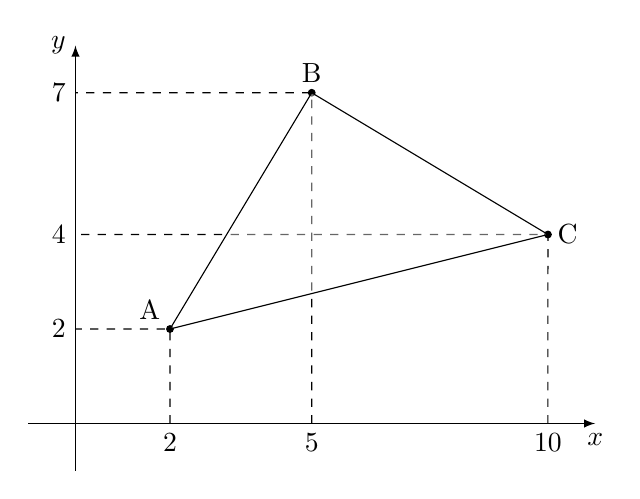
\begin{tikzpicture}[scale=0.6]
      \coordinate (A) at (2, 2);
      \coordinate (B) at (5, 7);
      \coordinate (C) at (10, 4);
      \filldraw (A) circle (2pt);
      \filldraw (B) circle (2pt);
      \filldraw (C) circle (2pt);
      \draw[-latex] (-1, 0) -- (11, 0) node[below] {$x$};
      \draw[-latex] (0, -1) -- (0, 8) node[left] {$y$};
      \draw[dashed] (2, 0) node[below] {$2$}-- (A) -- (0, 2) node[left] {$2$};
      \draw[dashed] (5, 0) node[below] {$5$}-- (B) -- (0, 7) node[left] {$7$};
      \draw[dashed] (10, 0) node[below] {$10$}-- (C) -- (0, 4) node[left] {$4$};
      \draw[fill=white, fill opacity=0.4] (A) node[above left, fill opacity=1]{A}-- (B)   node[above, fill opacity=1]{B} -- (C)   node[right, fill opacity=1] {C} -- (A) --  cycle;
    \end{tikzpicture}
  \end{figure}

Sejam ainda \(a\), \(b\) e \(c\) as medidas dos lados opostos aos vértices \(A\), \(B\), e \(C\), respectivamente. Temos que:
\begin{align*}
    &a = \overline{BC} = \sqrt{(C_x - B_x)^2 + (C_y - B_y)^2} = \sqrt{(10 - 5)^2 + (4 - 7)^2} = 5,83\\
    &b = \overline{AC} = \sqrt{(C_x - A_x)^2 + (C_y - A_y)^2} = \sqrt{(10 - 2)^2 + (4 - 2)^2} = 8,25\\
    &c = \overline{AB} = \sqrt{(B_x - A_x)^2 + (B_y - A_y)^2} = \sqrt{(5 - 2)^2 + (7 - 2)^2} = 5,83\\
  \end{align*}
Observemos que:
\begin{align*}
    \sqrt{a^2 + c^2} = \sqrt{5,83^2 + 5,83^2}= \sqrt{68 } = 8,25 = b
  \end{align*}

Portanto, o triângulo \(ABC\) é retângulo em \(B\).
\fimSol

\begin{enumerate}[resume]
  \item Mostre que o triângulo com vértices $(1,1)$, $(3, 5)$ e $(10, -1)$ é isósceles.
\end{enumerate}

\iniSol

Sejam \(A = (1, 1)\), \(B = (3, 5)\), \(C = (10, -1)\) os vértices do triângulo, conforme mostrado na figura abaixo:

\begin{figure}[H]
  \centering
  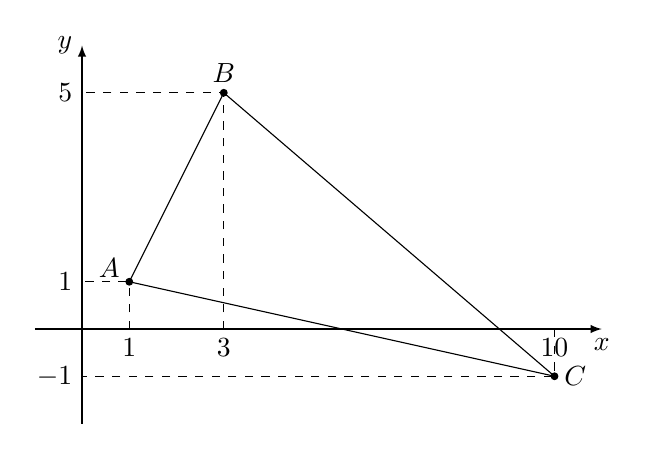
\begin{tikzpicture}[scale=0.6]
    \coordinate (A) at (1, 1);
    \coordinate (B) at (3, 5);
    \coordinate (C) at (10, -1);
    \filldraw (A) circle (2pt) node[left, yshift=5pt] {$A$};
    \filldraw (B) circle (2pt) node[above] {$B$};
    \filldraw (C) circle (2pt) node[right] {$C$};
    \draw (A) -- (B) -- (C) -- cycle;
    \draw[-latex] (-1, 0) -- (11, 0) node[below] {$x$};
    \draw[-latex] (0, -2) -- (0, 6) node[left] {$y$};
    \draw[dashed] (1, 0) node[below] {$1$} -- (1, 1) -- (0,1) node[left] {$1$};
    \draw[dashed] (3, 0) node[below] {$3$} -- (3, 5) -- (0,5) node[left] {$5$};
    \draw[dashed] (10, 0) node[below] {$10$} -- (10, -1) -- (0,-1) node[left] {$-1$};
  \end{tikzpicture}
\end{figure}

Sejam ainda \(a\), \(b\) e \(c\) as medidas dos lados opostos aos vértices \(A\), \(B\) e \(C\), respectivamente. Temos que:
\begin{align*}
    &a = \overline{BC} = \sqrt{(C_x - B_x)^2 + (C_y - B_y)^2} = \sqrt{(10 - 3)^2 + (-1 - 5)^2} = 9,22\\
    &b = \overline{AC} = \sqrt{(C_x - A_x)^2 + (C_y - A_y)^2} = \sqrt{(10 - 1)^2 + (-1 - 1)^2} = 9,22\\
    &c = \overline{AB} = \sqrt{(B_x - A_x)^2 + (B_y - A_y)^2} = \sqrt{(3 - 1)^2 + (5 - 1)^2} = 4,47\\
  \end{align*}
Node \(a = b\). Então o triângulo \(ABC\) é isósceles.
\fimSol

\end{document}
